\begin{figure}[ht!]
    \centering
    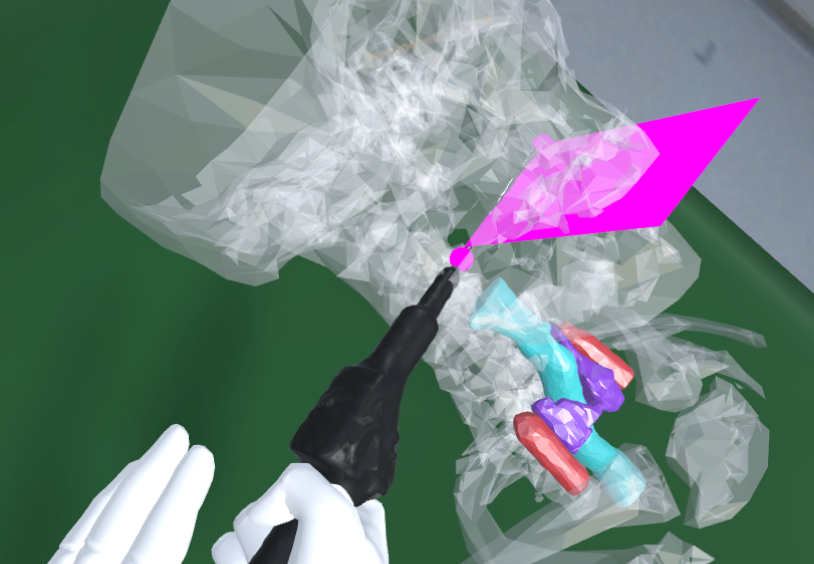
\includegraphics[width=\linewidth]{images/implementation/features/procedures/bonesaw.png}
    \caption{\label{fig::FeatureBoneSaw} Bonesaw Procedure}
\end{figure}

The sawing procedure is performed by picking up the bonesaw.
Touch the controller will show two indications to the user (Figure \ref{fig::FeatureBoneSaw}).
The procedure is performed by first pressing down the trigger button and then letting go of it.
When letting go of the trigger button, a two dimensianal plane is created in the three dimensional space by using four points.
Two of these points are created when pressing down, and the other two when letting go of the trigger button.
A plane is then created with which the user can reproduce the way in which the bonesaw has been moved.
Arbitrary cutting shapes can be created by breaking them down into two-dimensional shapes and performing multiple movements.